

\tikzset{every picture/.style={line width=0.75pt}} %set default line width to 0.75pt        
\begin{center}
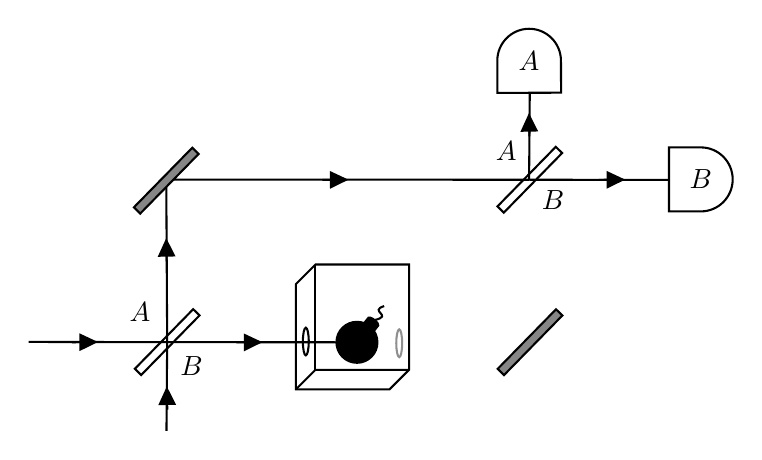
\begin{tikzpicture}[x=0.75pt,y=0.75pt,yscale=-1,xscale=1]
%uncomment if require: \path (0,300); %set diagram left start at 0, and has height of 300

%Shape: Rectangle [id:dp9015870766848293] 
\draw   (232.64,194.14) -- (260.76,165.42) -- (263.8,168.43) -- (235.68,197.15) -- cycle ;
%Straight Lines [id:da8378126329447328] 
\draw    (248.22,181.29) -- (247.88,224) ;


%Straight Lines [id:da4203005431788527] 
\draw    (181.51,181.2) -- (248.22,181.29) ;


%Straight Lines [id:da0243171970681888] 
\draw    (247.78,103.5) -- (248.22,181.29) ;


%Shape: Rectangle [id:dp6223611714942476] 
\draw   (407.34,115.91) -- (435.46,87.19) -- (438.5,90.2) -- (410.38,118.92) -- cycle ;
%Straight Lines [id:da6198680343533711] 
\draw    (248.58,181.29) -- (339.64,181.38) ;


%Straight Lines [id:da46097237064220464] 
\draw    (248.33,103.01) -- (422.78,103.05) ;


%Straight Lines [id:da9742962817963474] 
\draw    (422.92,103.05) -- (489.62,103.14) ;


%Straight Lines [id:da6938242067138403] 
\draw    (422.92,60.82) -- (422.59,103.53) ;


%Shape: Rectangle [id:dp9634903942334572] 
\draw  [color={rgb, 255:red, 0; green, 0; blue, 0 }  ,draw opacity=1 ][fill={rgb, 255:red, 134; green, 134; blue, 134 }  ,fill opacity=1 ] (232.19,116.35) -- (260.32,87.63) -- (263.36,90.64) -- (235.23,119.36) -- cycle ;
%Straight Lines [id:da5813104731210839] 
\draw    (202.27,181.35) -- (212.87,181.26) ;
\draw [shift={(214.87,181.24)}, rotate = 539.49] [fill={rgb, 255:red, 0; green, 0; blue, 0 }  ][line width=0.75]  [draw opacity=0] (8.93,-4.29) -- (0,0) -- (8.93,4.29) -- cycle    ;

%Straight Lines [id:da44635174735191185] 
\draw    (248.27,213.87) -- (248.09,204.64) ;
\draw [shift={(248.05,202.64)}, rotate = 448.87] [fill={rgb, 255:red, 0; green, 0; blue, 0 }  ][line width=0.75]  [draw opacity=0] (8.93,-4.29) -- (0,0) -- (8.93,4.29) -- cycle    ;

%Straight Lines [id:da0008306331435172787] 
\draw    (248,142.39) -- (247.82,133.17) ;
\draw [shift={(247.78,131.17)}, rotate = 448.87] [fill={rgb, 255:red, 0; green, 0; blue, 0 }  ][line width=0.75]  [draw opacity=0] (8.93,-4.29) -- (0,0) -- (8.93,4.29) -- cycle    ;

%Straight Lines [id:da07946196970039154] 
\draw    (322.96,103.14) -- (333.56,103.05) ;
\draw [shift={(335.56,103.03)}, rotate = 539.49] [fill={rgb, 255:red, 0; green, 0; blue, 0 }  ][line width=0.75]  [draw opacity=0] (8.93,-4.29) -- (0,0) -- (8.93,4.29) -- cycle    ;

%Straight Lines [id:da07206766467829073] 
\draw    (456.27,103.1) -- (466.87,103) ;
\draw [shift={(468.87,102.99)}, rotate = 539.49] [fill={rgb, 255:red, 0; green, 0; blue, 0 }  ][line width=0.75]  [draw opacity=0] (8.93,-4.29) -- (0,0) -- (8.93,4.29) -- cycle    ;

%Straight Lines [id:da618984745312871] 
\draw    (422.75,82.18) -- (422.57,72.95) ;
\draw [shift={(422.53,70.95)}, rotate = 448.87] [fill={rgb, 255:red, 0; green, 0; blue, 0 }  ][line width=0.75]  [draw opacity=0] (8.93,-4.29) -- (0,0) -- (8.93,4.29) -- cycle    ;

%Flowchart: Delay [id:dp8754933152186037] 
\draw   (490.01,87.47) -- (505.34,87.47) .. controls (513.81,87.47) and (520.68,94.38) .. (520.68,102.89) .. controls (520.68,111.41) and (513.81,118.31) .. (505.34,118.31) -- (490.01,118.31) -- cycle ;
%Flowchart: Delay [id:dp7631066454512347] 
\draw   (407.32,61.21) -- (407.27,45.79) .. controls (407.24,37.28) and (414.08,30.35) .. (422.55,30.32) .. controls (431.02,30.29) and (437.91,37.17) .. (437.94,45.69) -- (438,61.11) -- cycle ;
%Shape: Rectangle [id:dp0901747104841557] 
\draw  [color={rgb, 255:red, 0; green, 0; blue, 0 }  ,draw opacity=1 ][fill={rgb, 255:red, 134; green, 134; blue, 134 }  ,fill opacity=1 ] (407.45,194.18) -- (435.57,165.46) -- (438.61,168.47) -- (410.49,197.19) -- cycle ;
%Shape: Circle [id:dp21556459507248826] 
\draw  [fill={rgb, 255:red, 0; green, 0; blue, 0 }  ,fill opacity=1 ] (329.77,181.38) .. controls (329.77,175.92) and (334.19,171.5) .. (339.64,171.5) .. controls (345.1,171.5) and (349.52,175.92) .. (349.52,181.38) .. controls (349.52,186.83) and (345.1,191.25) .. (339.64,191.25) .. controls (334.19,191.25) and (329.77,186.83) .. (329.77,181.38) -- cycle ;
%Flowchart: Stored Data [id:dp7749919190363537] 
\draw  [fill={rgb, 255:red, 0; green, 0; blue, 0 }  ,fill opacity=1 ] (349.91,173.29) -- (346.81,177.19) .. controls (347.14,176.78) and (346.34,175.61) .. (345.04,174.57) .. controls (343.74,173.54) and (342.42,173.03) .. (342.09,173.44) -- (345.19,169.54) .. controls (345.51,169.13) and (346.84,169.64) .. (348.14,170.67) .. controls (349.44,171.71) and (350.24,172.88) .. (349.91,173.29) -- cycle ;
%Curve Lines [id:da27499232782476213] 
\draw    (348.14,170.67) .. controls (357.52,168.42) and (345.02,166.42) .. (352.77,163.92) ;


%Shape: Cube [id:dp8083755578351033] 
\draw   (364.78,194.63) -- (355.37,204.03) -- (310.25,204.03) -- (310.25,153.31) -- (319.66,143.9) -- (364.78,143.9) -- cycle ; \draw   (310.25,204.03) -- (319.66,194.63) -- (364.78,194.63) ; \draw   (319.66,194.63) -- (319.66,143.9) ;
%Shape: Ellipse [id:dp48925511756322826] 
\draw   (313.6,181) .. controls (313.6,177.32) and (314.23,174.33) .. (315.02,174.33) .. controls (315.8,174.33) and (316.43,177.32) .. (316.43,181) .. controls (316.43,184.68) and (315.8,187.67) .. (315.02,187.67) .. controls (314.23,187.67) and (313.6,184.68) .. (313.6,181) -- cycle ;
%Shape: Ellipse [id:dp9235217248592085] 
\draw  [color={rgb, 255:red, 0; green, 0; blue, 0 }  ,draw opacity=0.44 ][fill={rgb, 255:red, 0; green, 0; blue, 0 }  ,fill opacity=0 ] (358.6,181.83) .. controls (358.6,178.15) and (359.23,175.17) .. (360.02,175.17) .. controls (360.8,175.17) and (361.43,178.15) .. (361.43,181.83) .. controls (361.43,185.52) and (360.8,188.5) .. (360.02,188.5) .. controls (359.23,188.5) and (358.6,185.52) .. (358.6,181.83) -- cycle ;
%Straight Lines [id:da20174840319475407] 
\draw    (281.51,181.44) -- (292.11,181.35) ;
\draw [shift={(294.11,181.33)}, rotate = 539.49] [fill={rgb, 255:red, 0; green, 0; blue, 0 }  ][line width=0.75]  [draw opacity=0] (8.93,-4.29) -- (0,0) -- (8.93,4.29) -- cycle    ;


% Text Node
\draw (259.93,192.77) node   {$B$};
% Text Node
\draw (235.17,166.66) node   {$A$};
% Text Node
\draw (411.53,89.42) node   {$A$};
% Text Node
\draw (434.19,112.76) node   {$B$};
% Text Node
\draw (505.34,102.89) node   {$B$};
% Text Node
\draw (422.61,45.74) node   {$A$};


\end{tikzpicture}
\end{center}